\chapter{Visualisation implementation of the Improved Kepler Visualisation Tool
(IKVT)}\label{C:imp}
This chapter discusses the implementation of the visulisation using the designs
from Chapter \ref{C:sd} to fulfill the requirements of this project.
It details the tools used, the deliverable features
produced, and the problems encountered. 

\section{Tools and Artifacts Used}
\subsection{Keyboard \& Mouse System}
In addition to Processing there was an additional open-source
library required for effective user interface components called ControlP5
\cite{controlp5}. This library provides customisable and intuitive user
interface components. It allows for the creation of visually appealing and
precisely
aligned interactive GUI components.

\subsection{Microsoft Kinect System}
For the Microsoft Kinect version of IKVT two additional libraries were required
to integrate the Kinect sensor
with Processing, these were:
\begin{enumerate}
 \item NITE \cite{nite}.
 \item SimpleOpenNi \cite{simpleopenni}.
\end{enumerate}
These libraries provided drivers to run the Kinect sensor in Processing
(SimpleOpenNi) as well
as basic gesture recognition and body tracking (NITE). However these libraries
were
opensource options due to the official Microsoft Kinect SDK not being compatible
with
Processing. This meant the gesture recognition was not as user friendly or
effective as the
official libraries. The effect of this was that the gesture tracking used in the
system had to be created sup-optimally from the open-source libraries which took
more time and resources. 

\section{Implementation of IKVT}

IKVT displays all 2234 exoplanets
in the Kepler exoplanets dataset \cite{dataset}. Each of these exoplanets are
represented as coloured
ellipses, of which the colour and size are representative of the exoplanets
temperature and size respectively. IKVT displays all of these exoplanets as if
they are orbiting a single star. In reality this would result in planetary
collisions, but in this visualisation provides users with a way to effectively
make observations and comparisons about each of the exoplanets in a single
view. 

There are two panels that make up the visualisation: the visualisation panel,
and the control panel. The visualisation panel is where the exoplanets
are displayed along with a text box describing the state of the visualisation
to
keep the user informed. The control panel contains all of the interactive
components that the user can use to change the state of the visualisation. The
components it contains are; two text areas that can be used interchangeably to
display information about selected planets (Requirment 1), four range sliders
(Requirment 4) shown in Figure 
\ref{fig:sliders} that are used to
filter the exoplanets as discussed previously, and eight buttons to toggle the
state of the visualisations. These buttons are ``Sort by KOI'', ``Sort by Temp'',
``Sort by Size'', ``Sort by ESI'', ``Change View'', ``Suns Habitable Zone'', ``Pause'',
and ``Unsort'' as shown in Figure: \ref{fig:buttons}. 

\begin{figure}[H]
  \centering
      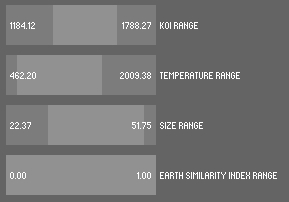
\includegraphics[width=0.6\textwidth]{images/sliders.jpg}
  \caption[Implementation of interactive range sliders]{Implementation of
interactive range sliders a various stages of filtering. The light grey bar in
the center of the sliders is the range of the attributes selected to filter by.
These can be modified by clicking and dragging on either end of the filter to
change the ranges, or selecting the middle to move the selected range up and
down the continuum}
  \label{fig:sliders}
\end{figure}

\begin{figure}[H]
  \centering
      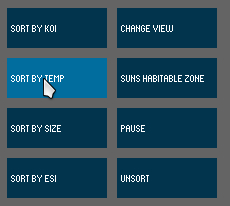
\includegraphics[width=0.6\textwidth]{images/buttons.jpg}
  \caption[Implementation of interactive buttons]{Implementation of interactive
buttons, each one of which corresponds to a key functionality in the
visualisation}
  \label{fig:buttons}
\end{figure}

Detailed information can be accessed about each exoplanet by clicking on them in
the main visualisation window to
make a selection. To do this a user can click on any of the orbiting exoplanets.
The effect of this selection is that a text box will have further textual
information about the selected exoplanet appended to it. In addition to this
users have the option of clicking a button labeled ``Compare''. This allows
the user the option to select another exoplanet so that its information is
appended to a second text area (Requirment 2). This can be seen in Figure
\ref{fig:textBoxes}. 
\begin{figure}[H]
  \centering
      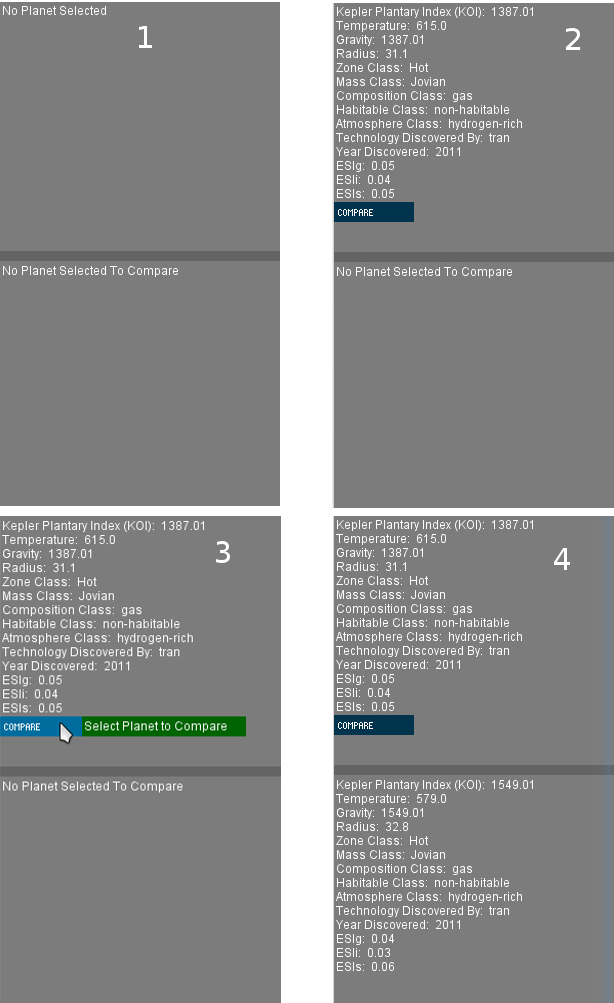
\includegraphics[width=0.7\textwidth]{images/textBoxes.jpg}
  \caption[Implemented text areas in each possible state]{Implemented text areas
in each possible state, Stage 1: No selection has been made so boxes are empty,
Stage 2: A single exoplanet has been selected and its information is displayed
as well as the option to compare, Stage 3: The user has chosen to compare the
selected exoplanet to another, Stage 4: A second exoplanet has been seleced and
its information added to the second text area.}
  \label{fig:textBoxes}
\end{figure}
When a user is unable to accurately select an
exoplanet due to the clustering or
overlapping of exoplanets they can move the camera around in space to gain a
better viewing position. If this is not
enough, the user can use a set of range selectors to filter the exoplanets
displayed, as shown in Figure \ref{fig:zoomFilter}. The exoplanets can be
filtered by their KOI,
temperature, size, and ESI. These filters allow for
users to fine tune the exoplanets they wish to view, thus allowing them to work
with small multiples rather than the entire dataset. Using
these filters also causes a zooming effect to occur as exoplanets are filtered
out.
This zooming occurs each time the filters are changed as the exoplanets spread
out vertically and allows more space between them to make selections.

\begin{figure}[H]
  \centering
      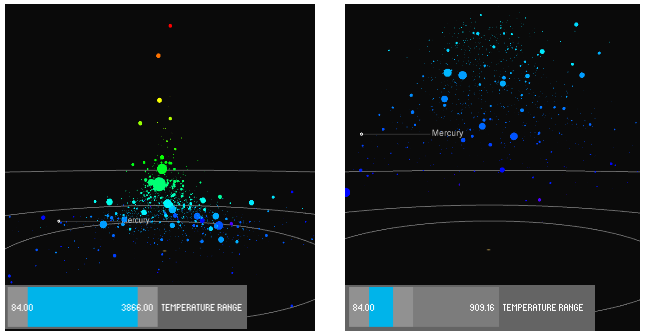
\includegraphics[width=0.8\textwidth]{images/zoomFilter.png}
  \caption[Zooming effect provided by filtering]{The above images display the
zooming effect provided by filtering. In the left image we can see that the
filters have not been used yet and all exoplanets are present which causes
clustering. In the right image the range has been  shrunk to filter out hot
exoplanets. This causes the colder planets to take up the space that was
originally occupied by all exoplanets which allows them to spread out.}  
    \label{fig:zoomFilter}
\end{figure}

The existing Kepler Visualisation Tool allowed users to sort the exoplanets on
the Y axis by their temperature and size. In IKVT this has been extended to
allow sorting by KOI and ESI (Requirment 3)as shown in Figure \ref{fig:ESIKOI}.


\begin{figure}[H]
  \centering
      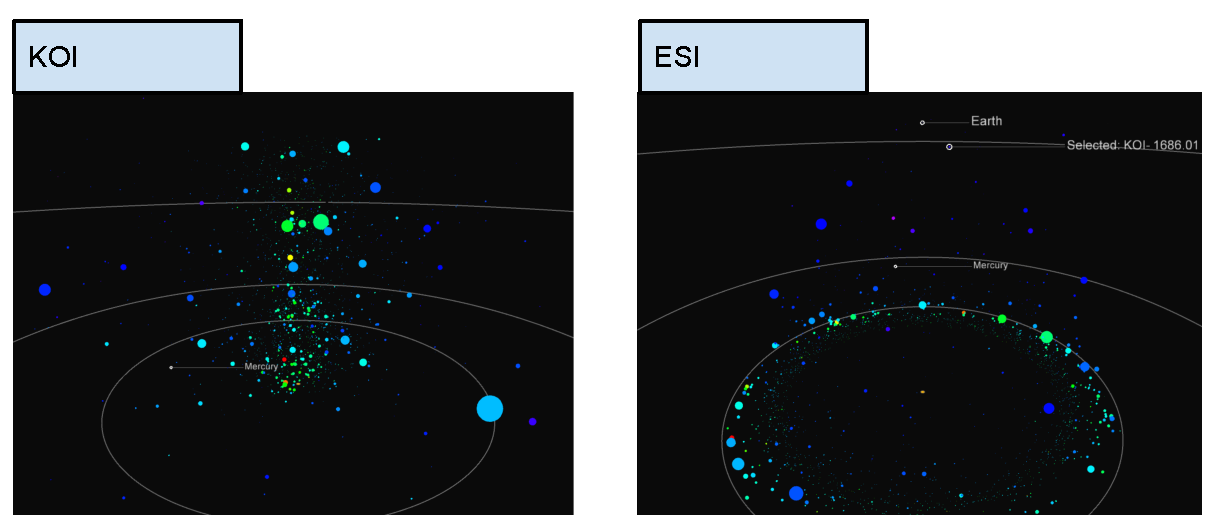
\includegraphics[width=1\textwidth]{images/ESIKOI.pdf}
  \caption[Implementation of sort by KOI and ESI]{The above images display the
implementation of sort by KOI and ESI. The left image shows the exoplanets sorted on the Y axis
by their KOI, this allows users to get an idea of which exoplanets share a solar
system as they will have similar KOI values. In the right image exoplanets are
sorted by their ESI on both the Y and X axis so that planets closer to the
center and the top are most similar to Earth}  
    \label{fig:ESIKOI}
\end{figure}

When a exoplanet is selected it is important that the user gets feedback about
what they have done. In IKVT this happens in the form of the selected exoplanet
becoming larger and a white outlining ring expanding out to encircle it. In
addition to this a label appears to the right of the exoplanet stating the
KOI. 

\begin{figure}[H]
  \centering
      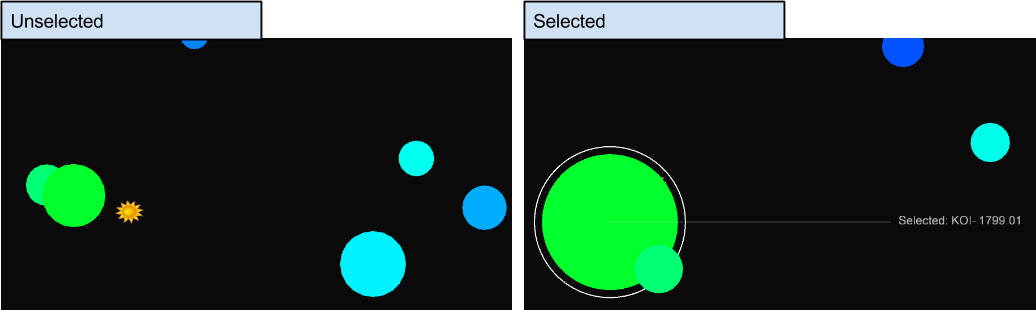
\includegraphics[width=1\textwidth]{images/selectedPlanet.jpg}
  \caption[Implentation of the exoplanet selection process]{The above images
display the implentation of the exoplanet selection process. We can see the
result of an exoplanet being selected, first the planet expands, then a white
circle expands out to outline it and a label appears to inform the user about
the exoplanet they selected.}  
    \label{fig:selectedPlanet}
\end{figure}

Another effect of a user making a selection is that all exoplanets that share
the same star as the selected exoplanet also become highlighted in the
same way as outlined above. The only difference is that in the label to the
right
of each exoplanet the message now informs the user that it has the ``Same
Star'' as displayed in Figure \ref{fig:sameStar}.

\begin{figure}[H]
  \centering
      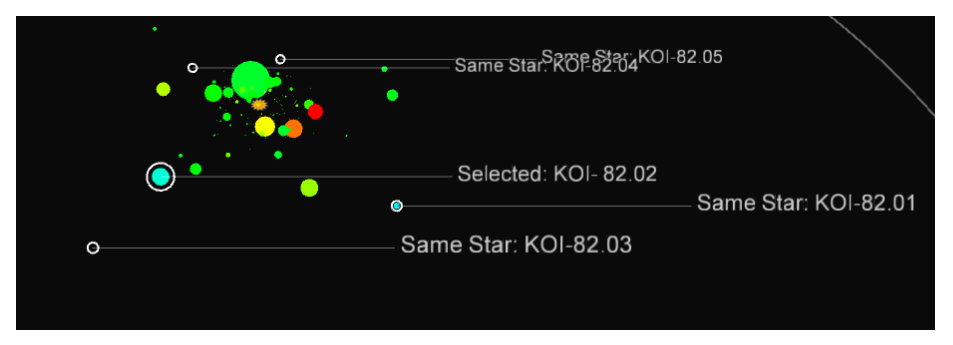
\includegraphics[width=1\textwidth]{images/sameStar.png}
  \caption[Implementation of exoplanets in the same solar system]{This image
displays how the planets in the same solar system as a selected planet become
highlighted in the same way but with a different label.}  
    \label{fig:sameStar}
\end{figure}


To display the Goldilocks zone of selected exoplanets coloured rings appear to
display the habitable
and inhabitable zones of the star (Requirment 5). Each time a new planet is
selected the
coloured rings change to represent the newly selected exoplanet's star, this can
be seen in Figure
\ref{fig:habitable}. In addition to the coloured rings the selected planet also
becomes highlighted
and all of the other exoplanets become transparent making it stand out to help users understand
whether it is in a habitable zone or not.

\begin{figure}[H]
  \centering
      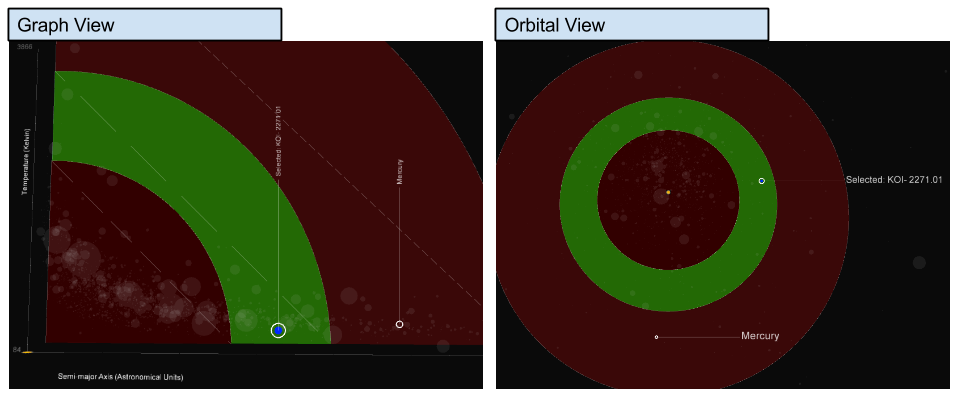
\includegraphics[width=1\textwidth]{images/habitable.png}
  \caption[Implementation of Goldilocks zones]{This image displays the
implementation the view Goldilocks zones feature which show how the coloured
rings are used, and how the planets relation to them infers their habitability.}
  
    \label{fig:habitable}
\end{figure}

Each of these implemented elements need to be visually apparent and intuitive to
use to ensure that the system can be
easily used without prior experience. This is done by providing clearly
labeled interactive elements and tooltips explaining what they
do as in Figure \ref{fig:tooltip}. These tooltips are widely used as a method of
informing a
user about the purpose of an item by hovering over it removing the need to
click on a button to discover its effect.

\begin{figure}[H]
  \centering
      
\includegraphics[width=0.8\textwidth]{images/tooltip.jpg}
  \caption[Tooltip on hover]{This image displays the implemented tooltips which
allow users to hover over interactive elements to discover what they do which
removes the need to
click on a button to discover its effect}
  \label{fig:tooltip}
\end{figure}

Due to the need for effective user interaction with the visualisation, a window
is required to house all of the components discussed above. Having this window
spatially separated from the main visualisation window means that users will not
be drawn away from the visualisation by overlapping and intrusive controls. Each
of the controls discussed above are included in this panel as shown below in
Figure \ref{fig:nav}.

\begin{figure}[H]
  \centering
      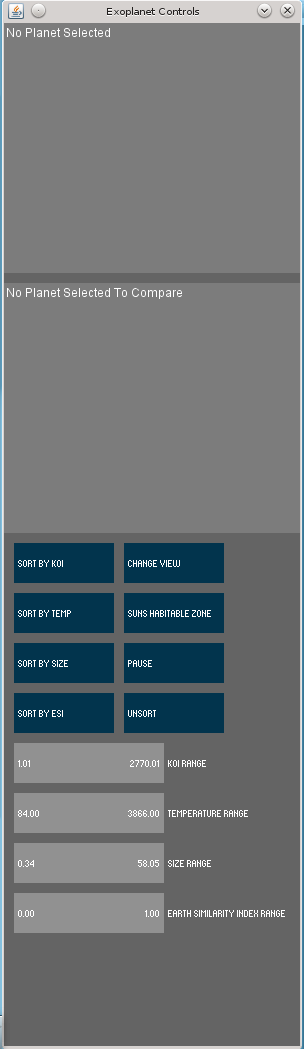
\includegraphics[width=0.3\textwidth]{images/nav.png}
  \caption[Implementation of Control Panel]{Shows the implemented Control Panel
that contains all of the interactive components discussed previously.}
  \label{fig:nav}
\end{figure}

At first the visualisation was laid out so that the control panel took up a
300 pixel strip along the bottom of the screen with the main visualisation
window
taking up the rest of the space as in Figure \ref{fig:layoutOld}.
 This was found to be unsuitable as the majority of the interaction and
animation of visualisation elements occurs
in the center of the window which this layout did not effectively utilise as it
caused a low aspect ratio that made the top and bottom of the visualisation to
be
cut off. It
was more effective to use two vertical columns as in Figure \ref{fig:layoutNew}
to view and control the visualisation. This is because
the higher aspect ratio allowed more of the content to be seen on the
screen at once as the majority of computer screens have a
wide aspect ratio. As you can see by comparing the two figures, Figure
\ref{fig:layoutNew} cuts off less of the visualisation and so is a more suitable
choice.

\begin{figure}[H]
  \centering
      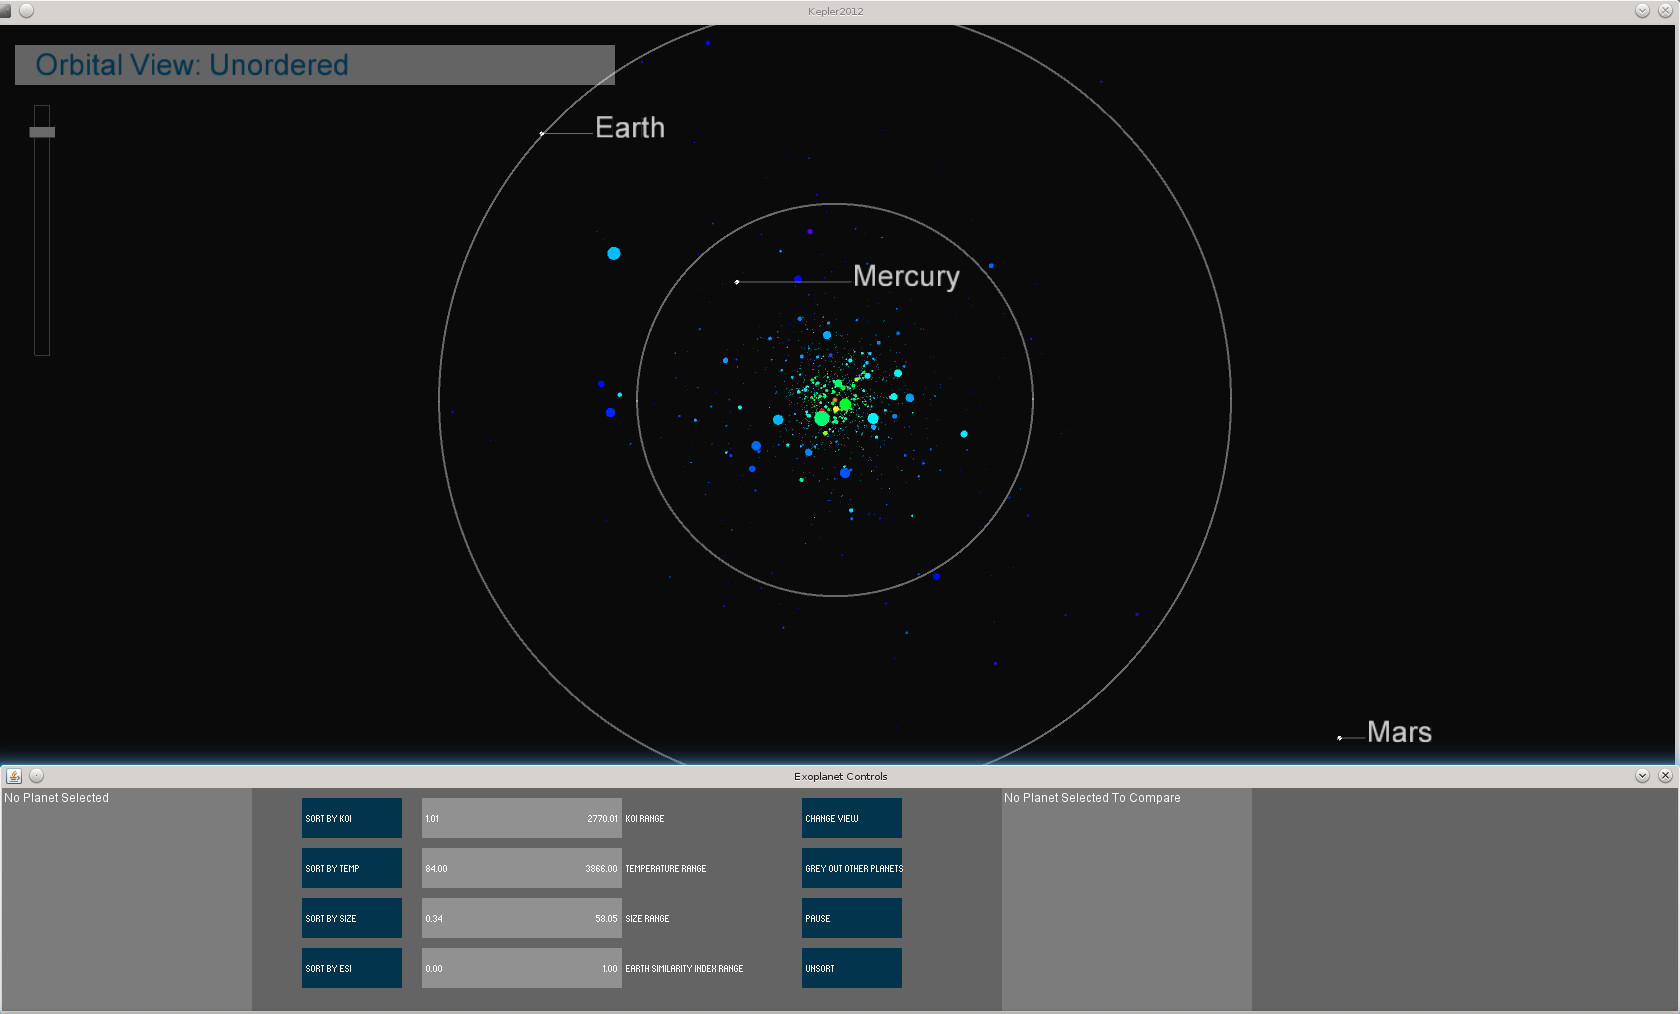
\includegraphics[width=0.8\textwidth]{images/layout_horizontal.jpg}
  \caption[Original Horizontal Layout]{Original Horizontal Layout that had an
unsuitable aspect ratio that occluded part of the visualisation.}  
    \label{fig:layoutOld}
        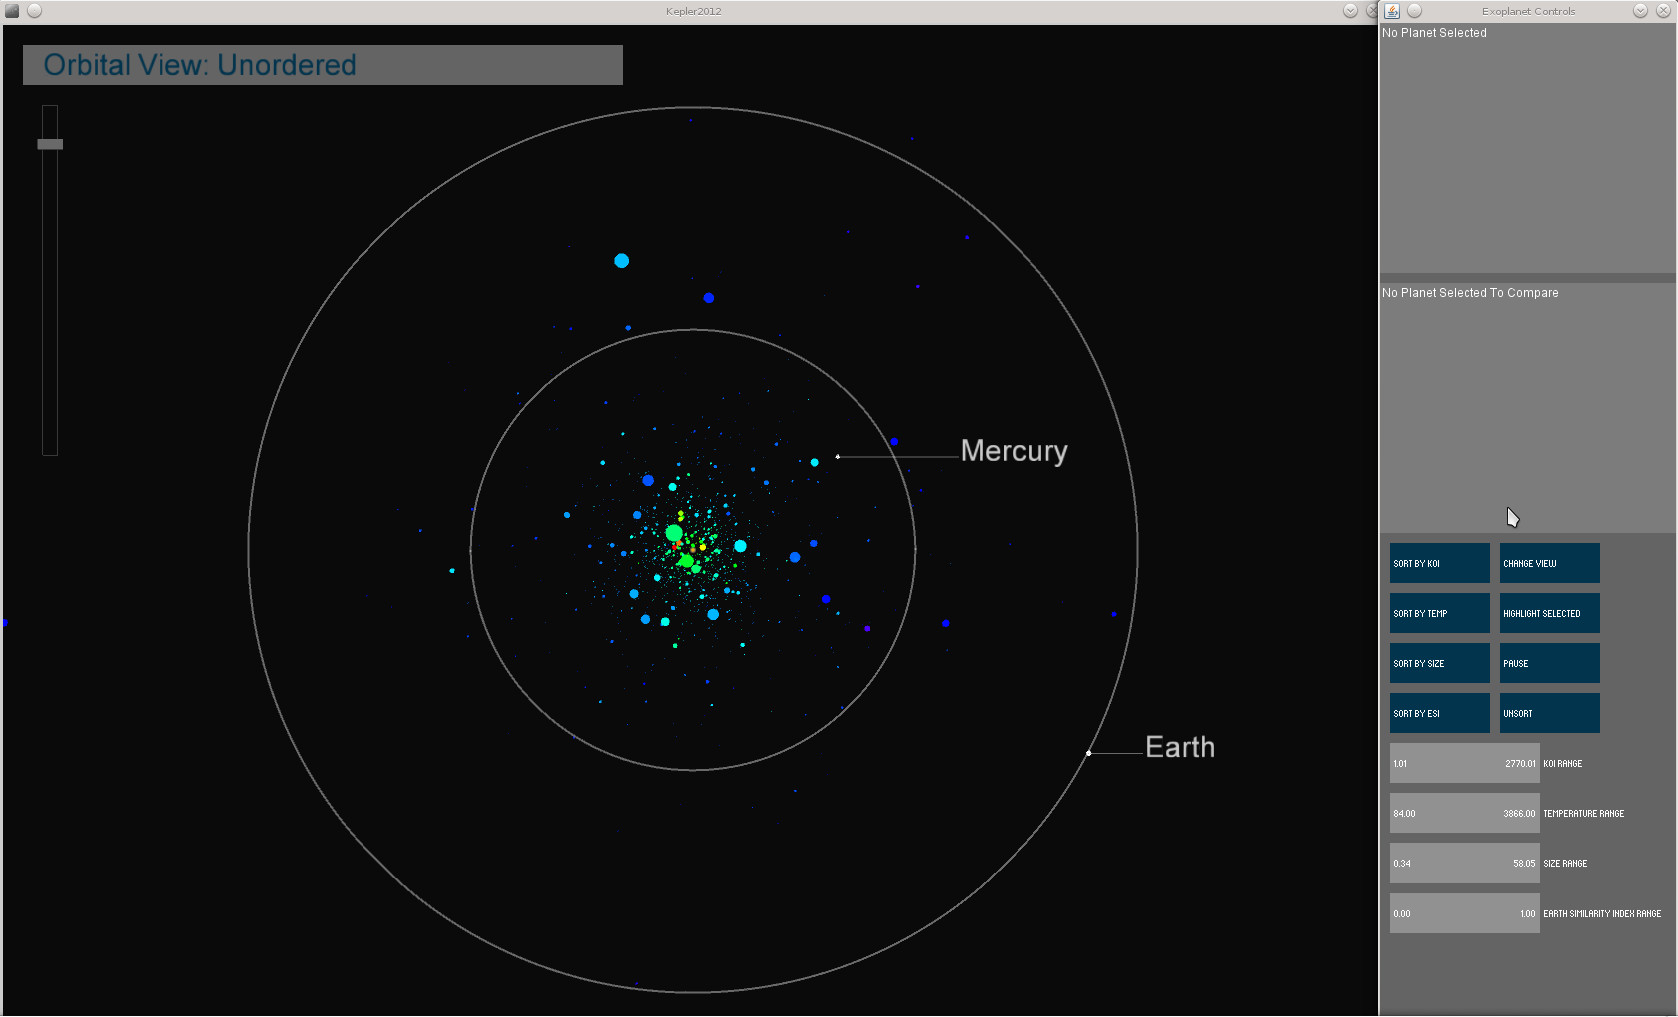
\includegraphics[width=0.8\textwidth]{images/layout_vertical.jpg}
  \caption[Improved Vertical Layout]{Improved Vertical Layout that had a higher
aspect ratio that did not hide any of the visualisation.}
  \label{fig:layoutNew}
\end{figure}

The Kinect Sensor system uses all of the features discussed above and extends it
by incorporating in gesture based control by utilising a Microsoft Kinect
sensor. Incorporate these gesture based controls was completed by specifying
gestures are detected by the visualisation which in turn modifies its state. 

\begin{figure}[H]
  \centering
      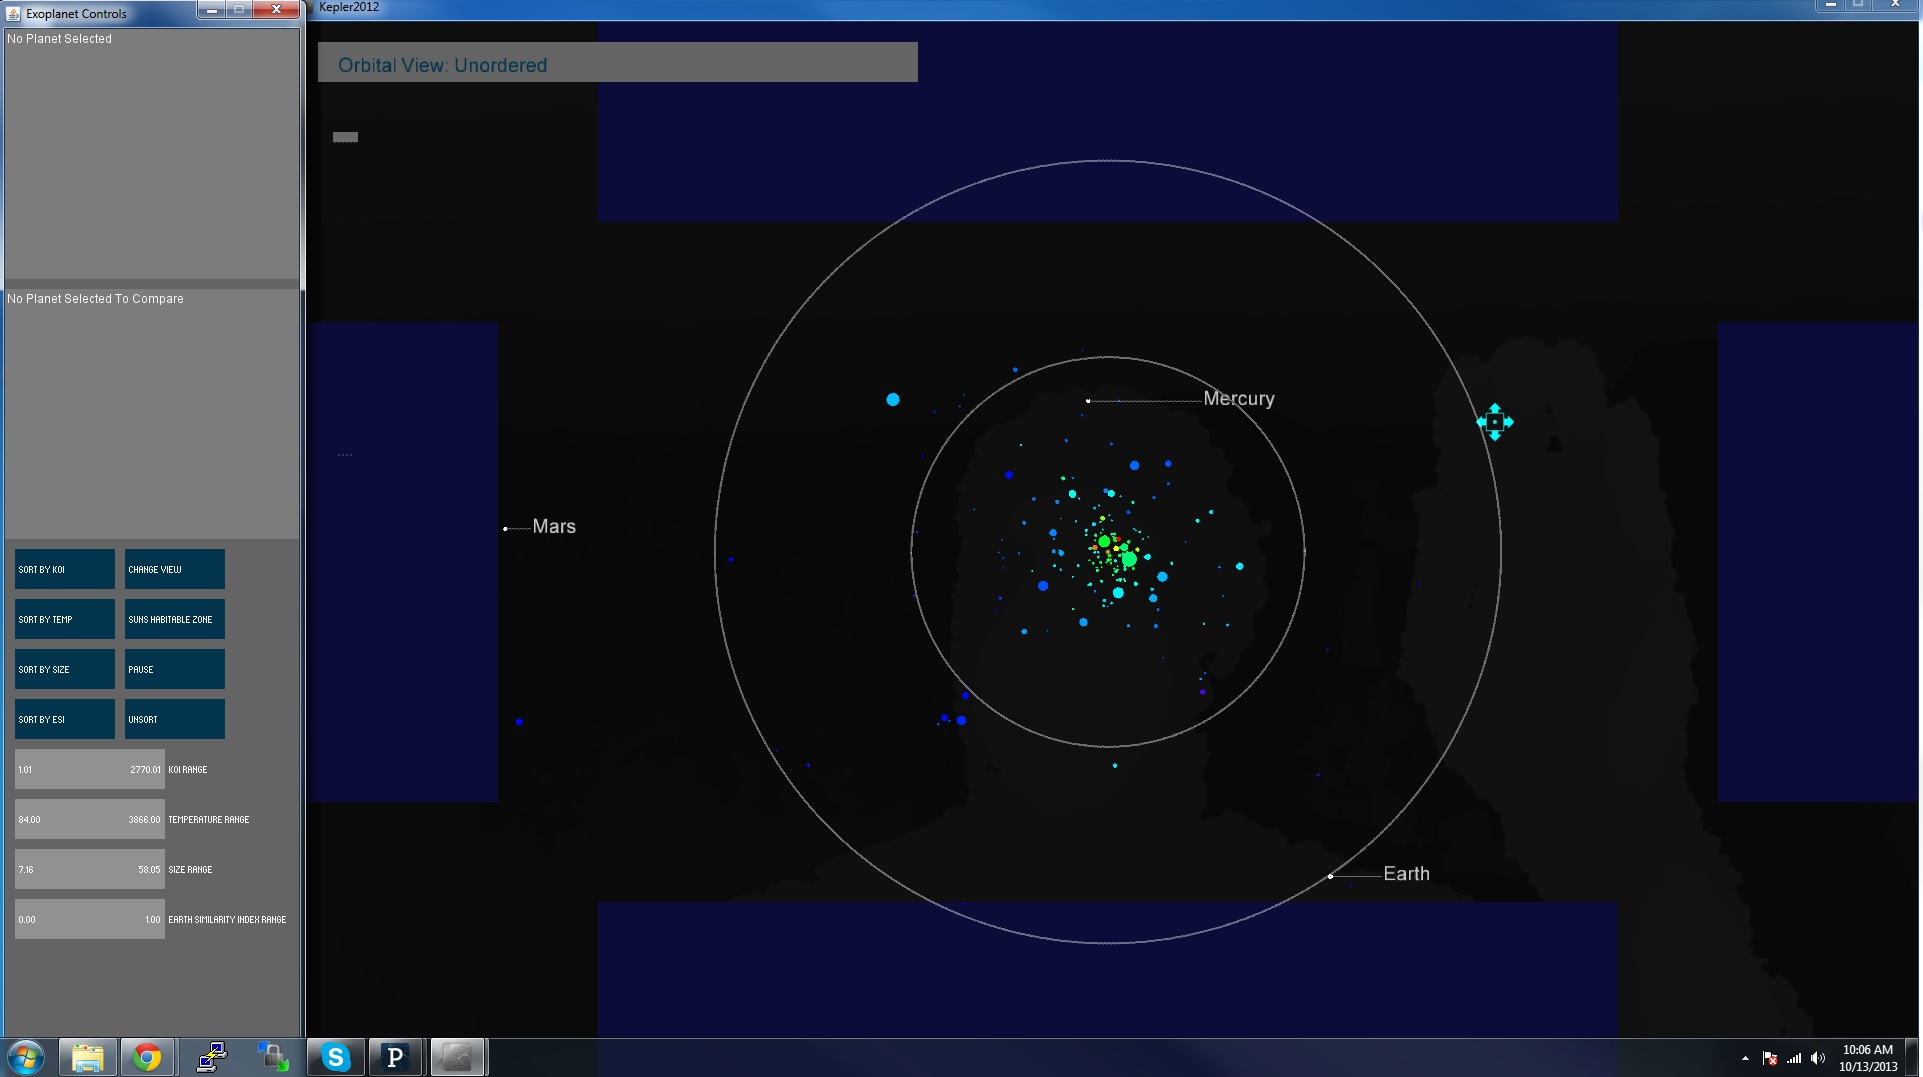
\includegraphics[width=0.8\textwidth]{images/full.jpg}
  \caption[Kinect system visualisation window]{Kinect system visualisation
window with the basic cursor visible on the outline of the users hand. Also
visible are the blue areas on the outsides of the visualisation indicating how
to perform gestures}
  \label{fig:left}
\end{figure}


As
shown in the solution design stage there were eight gestures that were needed
for the visualisation, each of which was implemented as described below
\begin{description}
 \item[1. Default cursor, hand is at rest or hovering over a planet.]
 
\begin{figure}[H]
  \centering
      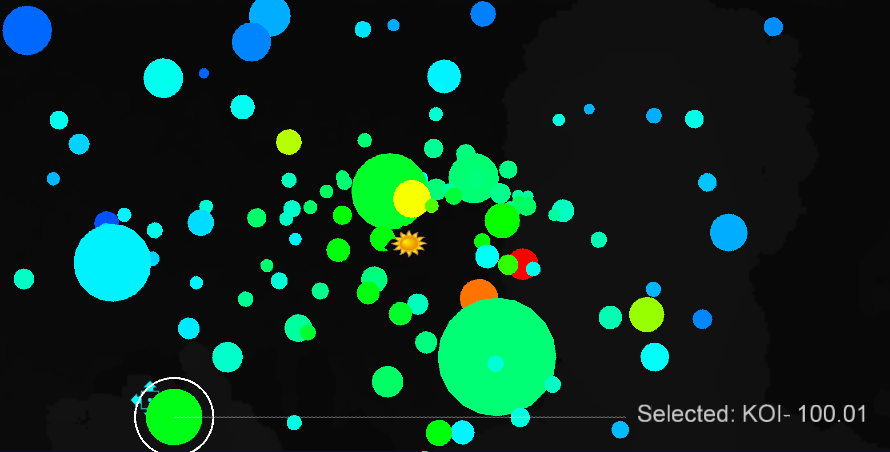
\includegraphics[width=0.8\textwidth]{images/select.PNG}
  \caption[Selecting a planet by gesture]{Selecting a planet by gesture by
hovering a hand over it. The basic cursor appears behind the selected planet.}
  \label{fig:left}
\end{figure}

 \item[2 \& 3. Panning up, hand is raised or panning down, hand is lowered.]
 \begin{figure}[H]
  \centering
      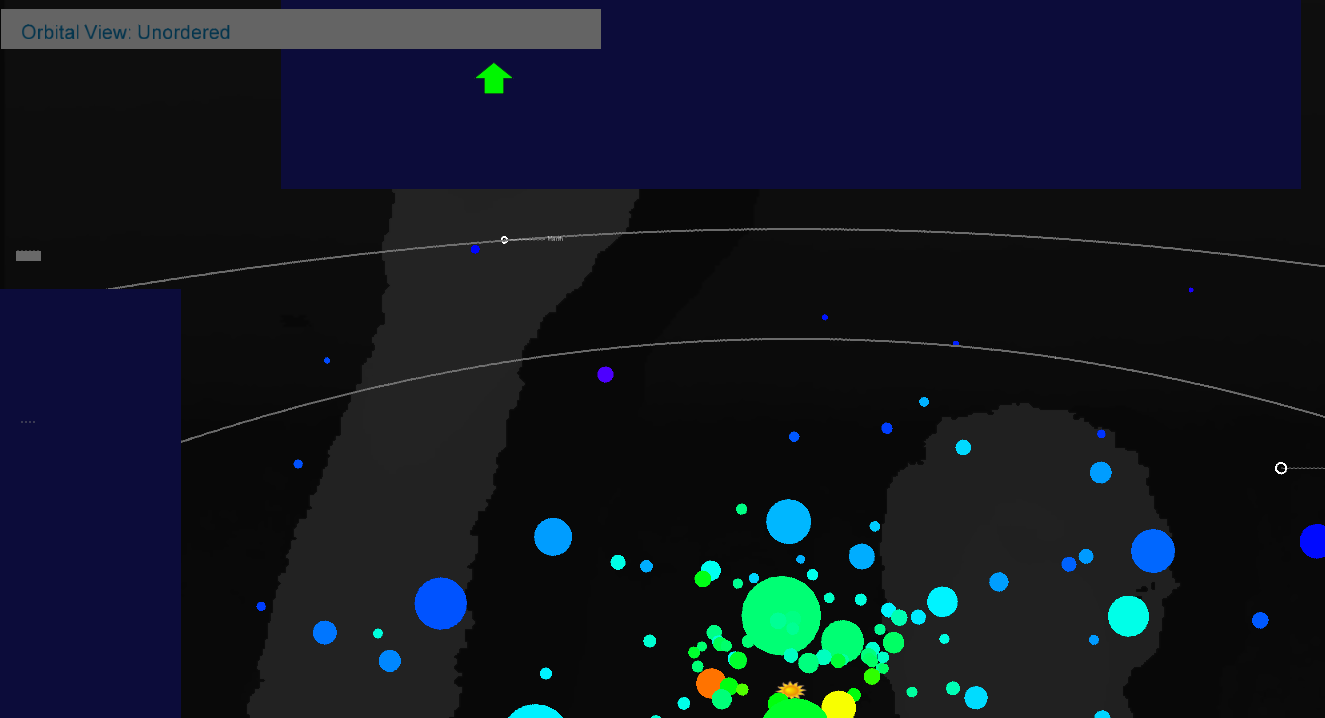
\includegraphics[width=0.8\textwidth]{images/up.PNG}
  \caption[Panning the visualisation by raising hand]{Panning the visualisation
by raising hand to the top blue area. The cursor indicates the visualisation is
panning up.}
  \label{fig:up}
\end{figure}
 
 \item[4 \& 5. Rotating left, hand is to the left or rotating right, hand is to
the right.]
 
\begin{figure}[H]
  \centering
      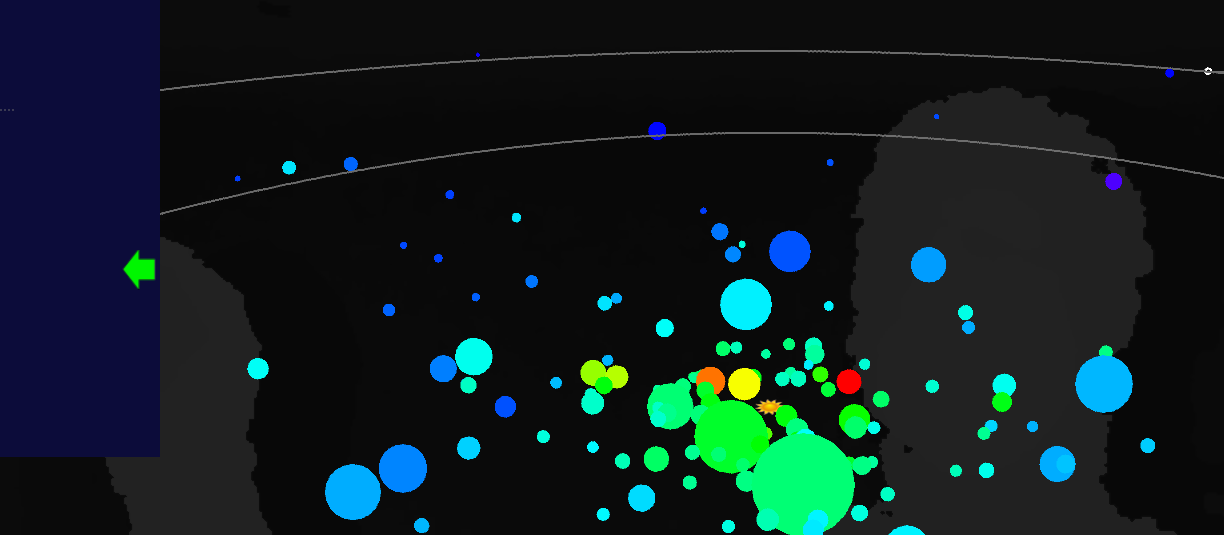
\includegraphics[width=0.8\textwidth]{images/left.PNG}
  \caption[Rotating visualisation be swiping hand]{Rotating visualisation be
swiping hand to the left of the screen. The cursor indicates the visualisation
is rotating left.}
  \label{fig:left}
\end{figure}

 \item[6. Zooming in, hand is pressed forward.]
 \begin{figure}[H]
  \centering
      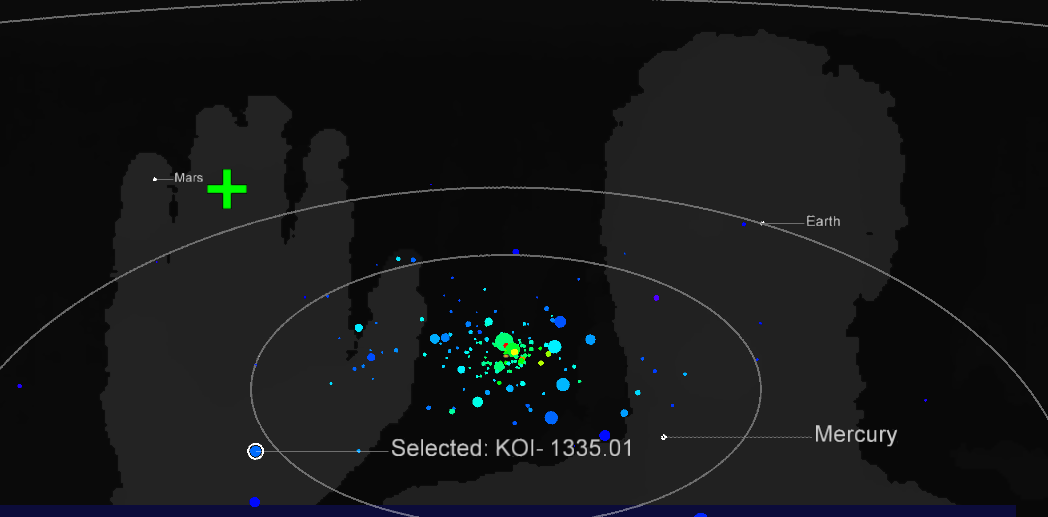
\includegraphics[width=0.8\textwidth]{images/in.PNG}
  \caption[Zooming in by pushing hand]{Zooming in by pushing hand towards the
screen. The cursor indicates the visualisation is zooming in.}
  \label{fig:in}
\end{figure}

 \item[7. Zooming out, hand is pulled backwards.]
 
\begin{figure}[H]
  \centering
      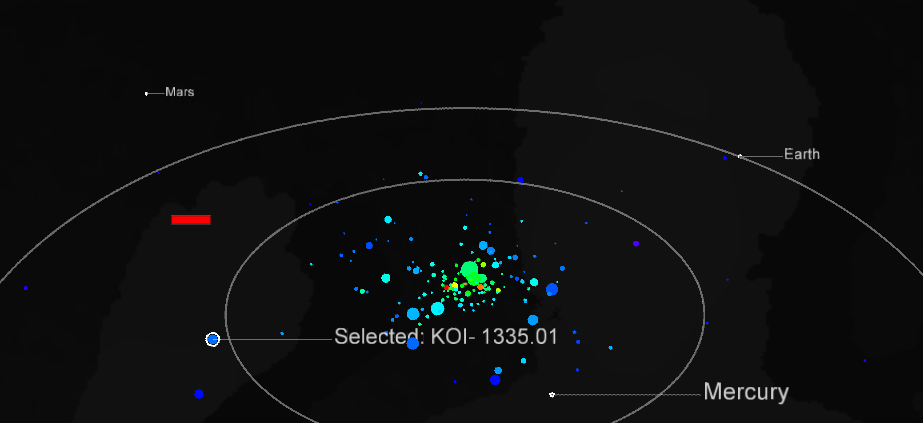
\includegraphics[width=0.8\textwidth]{images/out.PNG}
\caption[Zooming out by pulling hand]{Zooming out by pulling hand from the
screen. The cursor indicates the visualisation is zooming out.}
  \label{fig:out}
\end{figure}

\end{description}

In addition to this, the screen displays the user in relation to the
the visualisation, this is done by displaying a transparent outline of
the user in the background of the visualisation as can be seen in the above
figures. This is important as it gives the user a way to infer where they are
gesturing and as a way to show them that they are being detected by the system.
\\\\
Each of the features discussed were implemented using the designs created in
Chapter \ref{C:sd} to fulfill the functional requirements.
The visualisation IKVT that was created can successfully display planetary
information to convey knowledge to users (Requirement 1), allow exoplanets to be
compared against one another (Requirement 2), order exoplanets by their ESI and
by their KOI (Requirement 3), allows users to define ranges of planetary
attributes to filter which planets are displayed (Requirement 4), and view the
habitable zones of stars in
relation to the planets orbiting them (Requirement 5). These functionalities
are evaluated in the next chapter to ensure that they successfully fulfill the
functional requirements as previously stated, as well as the non functional
requirements that emphasises usability for users.




\section{Problems Encountered}

As this project builds upon a previous system, much of the existing code and
execution flow required modification. This required understanding of how the
system was originally built and designed. Because this system did not have any
unit or integration tests, going ahead without a comprehensive knowledge of the
core functionality would be have led to ineffective planning and errors being
introduced into the system. To address this, extra time and resources were
allocated to the requirements analysis and solution design stages of the
project.
\\\\
%Making use of tall of the data
Due to the number of elements that needed to be displayed on screen at any one
time (i.e. 2234 ellipses to represent the exoplanets), the load placed on the
system was very high. This uncovered a bug in
the Processing library in which the memory use of the visualisation would
periodically increase until it crashed due to an Out of Memory Exception. After
much experimentation with how to overcome this issue, I discovered that rather
than trying to render a native ellipse shape in processing, if I instead
rendered
a Scalable Vector Graphic this bug would not manifest. 
\\\\
Using the Processing framework meant using a non commercial IDE that is not
completely robust, for example when undoing multiple times in a row the file
being
modified would periodically become corrupted by lines of code being taken away
or inserted into the wrong locations. The solution to this issue was to ensure
that any changes were committed regularly to my repository on Github
\cite{github}. Doing this meant that if at any time a file became corrupted the
incorrect changes could be easily compared against the previous commit and
manually fixed. Any bugs found were reported in
the hopes that others using Processing in the future wouldn't need to address
them.
\\\\
The libraries used for gesture detection with the Kinect sensor were open-source
as this was the only way to get it to work with Processing. These open source
libraries did not have the functionality, documentation, and support that the
official Software Development Kit (SDK) that is available from Microsoft has
had. Whilst this was not a roadblock in terms of development it did mean that
more time was required for research and experimentation during implementation.
\\\\

